%
% File acl2020.tex
%
%% Based on the style files for ACL 2020, which were
%% Based on the style files for ACL 2018, NAACL 2018/19, which were
%% Based on the style files for ACL-2015, with some improvements
%% taken from the NAACL-2016 style
%% Based on the style files for ACL-2014, which were, in turn,
%% based on ACL-2013, ACL-2012, ACL-2011, ACL-2010, ACL-IJCNLP-2009,
%% EACL-2009, IJCNLP-2008...
%% Based on the style files for EACL 2006 by 
%%e.agirre@ehu.es or Sergi.Balari@uab.es
%% and that of ACL 08 by Joakim Nivre and Noah Smith

\newcount\Comments % 0 suppresses notes to selves in text
\Comments=1 % TODO: set to 0 for final version

\documentclass[11pt,a4paper]{article}
\usepackage[hyperref]{acl2020}
%\usepackage{times}
\usepackage{mathptmx}
\usepackage{latexsym}
\renewcommand{\UrlFont}{\ttfamily\small}

% for comments
\usepackage{color}
\usepackage{colortbl}
\usepackage{graphicx}
\usepackage{multirow}
\definecolor{darkgreen}{rgb}{0,0.5,0}
\definecolor{purple}{rgb}{1,0,1}
% \kibitz{color}{comment} inserts a colored comment in the text
\newcommand{\kibitz}[2]{\ifnum\Comments=1\textcolor{#1}{#2}\fi}
% add yourself here:
\newcommand{\nikolai}[1]{\kibitz{red}  {[Nikolai: #1]}}
\newcommand{\simon}[1] {\kibitz{blue} {[Simon: #1]}}
\newcommand{\asad}[1]{\kibitz{purple}  {[Asad: #1]}}

\usepackage{amsmath}
\usepackage{amssymb}
\usepackage{hhline}
\usepackage{tabularx}
\usepackage{subcaption,siunitx,booktabs}

\usepackage{tikz}
\usetikzlibrary{calc,shadows,shadows.blur}

\def\IosSevenSlider#1#2{
  \tikz[baseline=-0.1cm]{
    \coordinate (start) at (0,0);
    \coordinate (end) at (#1,0);
    \coordinate (mark) at ($(start)!#2!(end)$);
    \useasboundingbox (start|- 0,-.25) rectangle (end|- 0, .25);
    \draw[line width=0.4mm, line cap=round, blue!50!cyan] 
       (start) -- (mark) edge[lightgray] (end);
    \node[fill=white, draw=lightgray, very thin,
      blur shadow={shadow xshift=0pt, shadow opacity=20, shadow yshift=-0.9mm,
             shadow blur steps=6, shadow blur radius=0.3mm},
      circle, minimum size=0.25cm, inner sep=0pt] at (mark) {};
  }
}


\newcommand{\R}{\mathbb{R}}

% This is not strictly necessary, and may be commented out,
% but it will improve the layout of the manuscript,
% and will typically save some space.
\usepackage{microtype}

\aclfinalcopy % Uncomment this line for the final submission
%\def\aclpaperid{***} % Enter the acl Paper ID here

%\setlength\titlebox{5cm}
% You can expand the titlebox if you need extra space
% to show all the authors. Please do not make the titlebox
% smaller than 5cm (the original size); we will check this
% in the camera-ready version and ask you to change it back.

\newcommand\BibTeX{B\textsc{ib}\TeX}

\title{When an image tells a story: the role of visual and semantic information for generating paragraph descriptions}

\author{Nikolai Ilinykh \space\space\space\space\space\space\space Simon Dobnik\\
 Centre for Linguistic Theory and Studies in Probability (CLASP) \\
 Department of Philosophy, Linguistics and Theory of Science (FLoV) \\
 University of Gothenburg, Sweden \\
 \texttt{nikolai.ilinykh,simon.dobnik@gu.se} }

\date{}

\begin{document}
\maketitle
\begin{abstract}

  Generating multi-sentence image descriptions is a challenging task, which requires a good model to produce coherent and accurate paragraphs, describing salient objects in the image. % In this paper,
We argue that multiple sources of information are beneficial when describing visual scenes with long sequences. These include: (i) perceptual information and (ii) semantic (language) information about how to describe what is in the image. We also compare the effects of using two different pooling mechanisms on either a single modality or their combination. % As we demonstrate here,
We demonstrate that the model which utilises both visual and language inputs can be used to generate \textit{accurate} and \textit{diverse} paragraphs when combined with a particular pooling mechanism. The results of our automatic and human evaluation show that learning to embed semantic information along with visual stimuli into the paragraph generation model % to achieve better results
is not trivial, raising a variety of proposals for future experiments.

\end{abstract}

\section{Introduction}\label{sec:introduction}

The quality of automatically generated image captions \cite{bernardi2016automatic} has been continuously improving as evaluated by a variety of metrics.
These improvements include use of neural networks \cite{kiros14,vinyals2014tell}, attention mechanisms \cite{xu2015attend,Lu2016} and more fine-grained image features \cite{anderson2017bottomup}.
More recently, a novel open-ended task of image paragraph generation has been proposed by \newcite{krause2016hierarchical}.
This task requires the generation of multi-sentence image descriptions, which are highly informative, thus, include descriptions of a large variety of image objects, and attributes, which makes them different from standard single sentence captions.
In particular, a good paragraph generation model has to produce descriptive, detailed and coherent text passages, depicting salient parts in an image.

When humans describe images, especially over longer discourses, they take take into account (at least) two sources of information that interact with each other: (i) perceptual information as expressed by visual features and (ii) cognitive reasoning that determines the communicative intent of the text and the use of language \cite{Kelleher:2020aa}.
Perceptual information mainly determines \emph{what} to refer to while the reasoning mechanisms tell us \emph{how} and \emph{when} to refer to it.
Both mechanisms interact: that a particular object is described at a particular point of discourse and with particular words depends not only on its perceptual salience but also whether that object should be referred to at that point of the story that the text is narrating which is its discourse salience.
Compare for example: ``two cows are standing in the field'', ``there are trees in the field'' and ``a few of them are close to the trees''.
The selection and the order of the relevant features are described by a cognitive mechanism of attention and memory \cite{Lavie:2004aa,Dobnik:2016ac}.

\begin{figure}[h]
\centering
 \fbox{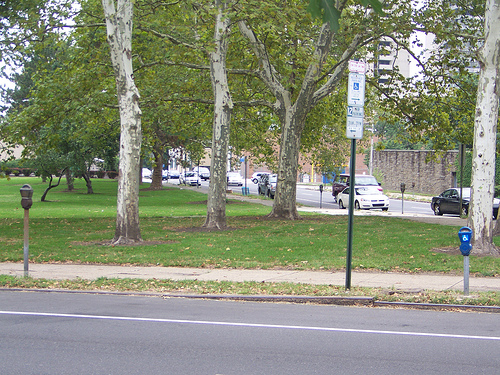
\includegraphics[width=\linewidth]{figures/example}}
 \caption{
 Example image with generated paragraphs from our models (incl. ground truth description):\\
 \textbf{HUMAN}: \textit{There are several cars parked along a street. There are many trees in a field in front of the street. There are small blue parking meters on the sidewalk next to the street.}\\
 \textbf{IMG+MAX} : \textit{There are several cars parked on the road. There are cars parked on the street. There are trees behind the street.}\\
 \textbf{LNG+MAX} : \textit{There are several cars on the street. There are trees on the street. There are trees on the street.}\\
 \textbf{IMG+LNG+MAX} : \textit{There are several cars on the street. There are two cars on the street. There are cars parked on the sidewalk.} \\
 \textbf{IMG+ATT} : \textit{There are several cars parked on the street. There are two cars parked on the road. There are two cars parked on the road.}\\
 \textbf{LNG+ATT} : \textit{There are several signs on the street. There are signs on the street. The pole is white.}\\
 \textbf{IMG+LNG+ATT} : \textit{There is a parking meter on a sidewalk. There are cars next to the street. There is a parking lot next to the street.} 
 }
 \label{example}
\end{figure}

In this paper, we investigate the interplay between visual and textual information (reflecting background knowledge about the world and communicative intent) and their ability to generate natural linguistic discourses spanning over several sentences.
% To improve on the first point, for each generated sentence we learn to attend to salient objects in the scene.,
Our primary research question is as follows: does % supply image paragraph models with
using both visual and linguistic information improve \emph{accuracy} and \emph{diversity} of generated paragraphs?
% We expect these types of input to be complementary in generating varied paragraphs.
We experiment with several types of inputs to the paragraph generator: visual, language or both.
We also investigate the effects of different kinds of information fusion between visual and textual information using either attention or max-pooling. % on image regions as a way of representing an image as a whole.
We demonstrate that multimodal input paired with attention on these modalities benefits model's ability to generate more diverse and accurate paragraphs.
Fig.~\ref{example} shows an image with generated texts from both human and our models.

We evaluate the accuracy and diversity of our paragraphs with both automatic metrics and human judgements.
We also argue that, as some previous work shows \cite{vanderlee2019}, \textit{n}-gram-based metrics might be unreliable for quality evaluation of generated texts.
The generated paragraph can be accurate as of the image, but because it does not match the ground truth, this would score low based on the automatic evaluation.
To provide a different view on paragraph evaluation, we asked humans to judge the subset of generated paragraphs across several criteria, more specifically described in Section~\ref{humaneval} and Appendix~\ref{sec:supplemental}.

% Additionally, we note that paragraphs must be \textit{accurate} in describing an image.
% For completeness, we also report results of the automatic evaluation, showing that automatic metrics, which aim to measure \textit{accuracy} of paragraphs rather than \textit{diversity}, do not necessarily pick the most diverse paragraph as the most accurate and vice versa.

% SD 2020-08-28 13:03:38 +0200: I would argue that automatic measures also do not capture accuracy. This is because most of them are based on keyword matching. We might generate an accurate description but because it does not match the ground truth this is counted as bad choice. I think our AMT experiment reflects both accuracy and diversity.
% Nikolai: that's a good point, I think something similar was mentioned somewhere, but I will put it here for now.
% I have also added some points about importance of human evaluation based on INLG papers: this topic is hot for this particular conference, so I believe it makes sense to cite some of their work.

In language and vision literature, ``diversity'' of image descriptions has been mostly defined in terms of lexical diversity, word choice and \textit{n}-gram based metrics \cite{Devlin2015, Vijayakumar2016, Lindh2018, VanMiltenburg2018}.
% These criteria are focused on
In this work, the focus is on generating a diverse set of \textit{independent, one-sentence captions}, with each describing image as a whole.
Each of these captions might refer to identical objects due to the nature of the task ("describe an image with a single sentence").
Then, diversity is measured in terms of how different object descriptions are from one caption to another (e.g. a man can be described as a ``person'' or ``human'' in two different captions).
However, as argued above, a good image paragraph model must also introduce diversity at the sentence level, describing \textit{different scene objects} throughout the paragraph. % is what makes it more informative than single sentence captions.
Here, we define \textit{paragraph diversity} with two essential conditions.
First, a generative model must demonstrate the ability to use % many different
relevant words to describe objects without unnecessary repetitions (\emph{word-level diversity}).
Secondly, it must produce a set of sentences with relevant mentions of a variety of image objects in an appropriate order (\emph{sentence-level diversity}).

% SD 2020-08-28 13:26:03 +0200: We are adding the order to diversity here. One mioght argue that this deserves a separate heading but let us leave it this way.
% Nikolai: Yeah, we have never really paid that much attention to these two levels of diversity. Agreed, let's keep it like this for now.

Producing structured and ordered sets of sentences (e.g. \textit{coherent paragraphs}) has been a topic of research in NLG community for a long time with both formal theories of coherence \cite{grosz95,Barzilay2008} and traditional rule-based model implementations \cite{Reiter00buildingnatural,Deemter:2016aa}.
The coherence of generated text depends on several NLG sub-tasks: \textit{content determination (selection)}, the task of deciding which parts of the source information should be included in the output description, and \textit{text structuring (micro-planning)}, the task of ordering selected information \cite{Gatt2017}.
We believe that the hierarchical structure of our models reflects the nature of these tasks. First, the model attends to the image objects and defines both their salience and order of mention and then it starts to realise them linguistically, first as paragraph visual-textual topics and then as individual sentences within paragraphs.
% need more references about discourse structure
% cite ilinykh19 as an example of structured paragraphs
% \nikolai{more references about discourse structure are needed}

% SD 2020-08-28 14:07:33 +0200: Unfortunately, this does not fit here anymore. Find another place?
% More recently, \newcite{ilinykh19} collected the dataset of image description sequences (mini-discourses).
% These mini-discourses are especially useful for learning models which can plan and realise such ordered and structured data.


\iffalse
Humans are typically able to effortlessly describe real-world images when required: we easily identify objects, attributes and relations between them.
Diversity, richness and complexity of such human-produced image descriptions have been observed in several benchmark image description datasets, including MSCOCO \cite{lin2014microsoft,chen2015microsoft}, Flickr8k \cite{hodosh2013}, Flickr30k \cite{young-etal-2014-image}, Visual Genome \cite{krishnavisualgenome}.
These datasets were collected to address the task of automatic image description \cite{bernardi2016automatic}, a long-standing and active field of research, placed in intersection between computer vision and natural language processing (generation, in particular).
This problem of mapping visual data to text can be viewed as the specific example of one of the core goals of NLG: `translating' source data into a natural language representation.
In natural language generation community, the task of text generation has been typically divided into multiple sub-tasks, including \textit{content determination (selection)}, the task of deciding which parts of the source information should be included in the output description, and \textit{text structuring}, the task of ordering selected information \cite{Gatt2017}.
However, with the rise of neural networks in many NLP areas, the generation tasks are now seen as a continuous, non-modular process of automatically learning relations between input and expected output. Specifically, neural models of image captioning \cite{kiros14,vinyals2014tell} are trying to implicitly learn what is important about an image (content selection) and how this information should be structured in the generated caption (text structuring).
Such mechanisms as attention \cite{xu2015attend,anderson2017bottomup} further improve ability of the models to locate important parts in an image and utilise them for caption generation. Some recent advances in image captioning include application of transformer architecture \cite{vaswani2017attention,herdade2019image}.

% SD 2020-07-09 16:50:13 +0200: This is a very good introduction but probably rhe readers of the paper would already know this. We can shorten it later.

While it is clear that neural networks demonstrate good performance in generating \textit{well-structured} single-sentence image captions with \textit{relevant knowledge}, the problem of selecting and ordering information becomes significantly harder when generating multiple sentences for a single image. The corresponding task of
\textit{image paragraph generation} has been initially introduced in \newcite{krause2016hierarchical}, proposing the challenge of generating a text, consisting of several sentences that would form a coherent whole.
Most of the following work \cite{liang2017recurrent,chatterjee2018diverse,wang2019convolutional} has focused on \textit{generating} good, diverse and human-like paragraphs as measured by various automatic evaluation metrics like BLEU \cite{bleu} or CIDEr \cite{vedantam2014cider}.

In this paper we look at the different aspect of image paragraph generation and address the problem of \textbf{information order} in the multi-sentence image captioning setting.
% SD 2020-07-09 16:52:39 +0200: Here we could give an example of a picture and text and describe differences between sentences and therefore explain what we mean by the discourse.
We argue that utilising top-down knowledge (information about context available to the captioner) is beneficial for the task of image paragraph generation.
We show that the model conditioned on both low-level visual features and high-level top-down information is able to learn human-like distributions of attended objects, attributes and relations generated in the paragraph.
We introduce several image paragraph models based on the hierarchical paragraph generator \newcite{krause2016hierarchical} and also
demonstrate that using bottom-up information exclusively is not enough to learn good paragraph structure.
We employ transfer learning and use model pre-trained for the dense image captioning task \cite{densecap} to obtain representations of background information, which we treat as our top-down features.
We evaluate how close our models are compared to the human performance in terms of attending to objects in visual scenes in a particular order.

% SD 2020-07-09 16:54:27 +0200: Quite a few points here. We can streamline them at the end when we shape the final argument for the paper.
\fi

% multimodality
% \cite{barzilay-lee-2004-catching} 


\begin{figure*}[h]
 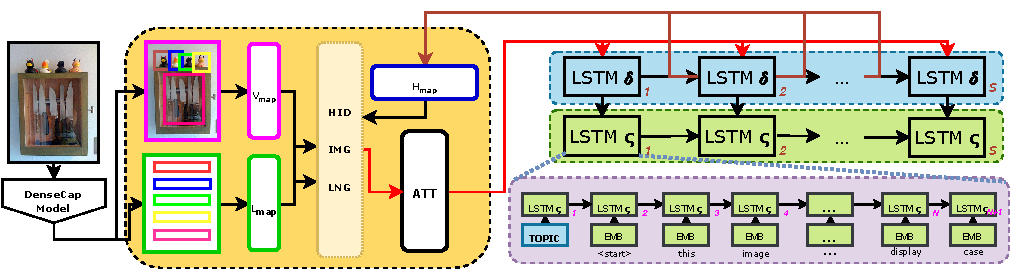
\includegraphics[width=\linewidth]{figures/model}
 \caption{Multimodal paragraph generator architecture.
 		The orange area on the left is the learned space where two modalities are attended to (vision in purple, language in green).
		The mapped features are concatenated together and passed to the attention mechanism, that outputs a vector which is used as an input to the discourse LSTM (in blue, marked with $\delta$).
		The attention module also uses the last hidden state of the discourse LSTM at each timestamp.
		The sentence LSTM (in green, marked with $\varsigma$) is given the sentence topic and word embeddings.
		Due to limited space, we omit the linear layer and the softmax layer which are used to predict the next word from the output of the sentence LSTM.}
 \label{fig:model}
\end{figure*}

\section{Approach}
\paragraph{Overview}
For our experiments we implement and adapt the hierarchical image paragraph model by \citet{krause2016hierarchical}.\footnote{The authors have not publicly released the code of their model and hence the model implementation is based on our interpretation of their paper.}
To prepare input features, we utilise the pre-trained model for dense captioning \cite{densecap} in two ways.
First, we use it to extract convolutional features of identified image regions.
We also use its hidden states from the RNN layer as language features.
In the original model, these states are used to generate region descriptions; therefore, these vectors represent semantic information about objects.
We construct \textit{a multi-modal space}, in which we learn mappings from both text and vision features.
Lastly, we concatenate both modalities and attend to them to form a multi-modal vector, which is used as an input to the paragraph generator.
%We fuse both modalities into a single vector represented by an affinity matrix, similar to \newcite{Xu2015} and \newcite{vqaLU16}. 
%This matrix captures similarities between visual and language representations for all combinations of regions.
% SD 2020-07-08 13:36:07 +0200: We need to say a bit more how the fusion is done.
%Then, the similarity vector is used by a two-level hierarchical paragraph generator.
Our paragraph generator consists of two components: discourse-level and sentence-level LSTMs \cite{lstm97}.
First, the discourse-level LSTM learns the topic of each sentence from the multi-modal representation, capturing information flow between sentences.
Second, each of the topics is used by sentence-level LSTM to generate an actual sentence.
Finally, all generated sentences per image are concatenated to form a final paragraph.
An overview of our model and a more detailed description is shown in Fig.~\ref{fig:model}.
Our model is different from the model by \newcite{krause2016hierarchical} in the following ways: (i) we use either max-pooling or attention in our models, (ii) we do not learn to predict the end of the paragraph, but generate the same number of sentences as we find in ground-truth paragraph per each image, (iii) we use semantic information about objects in the visual scene.
% SD 2020-08-30 22:50:59 +0200: Krause also does not use semantic information. --> added.
The focus of our work is not to improve on the results of \newcite{krause2016hierarchical} but to investigate the effects of different multi-modal fusion on the accuracy or the diversity of paragraph descriptions. % SD 2020-08-28 14:22:15 +0200: Added this sentence to emphasise our relation to Krause.
% SD 2020-08-28 14:18:35 +0200: But this is not the only difference from Krause. Here is a good point to say: Our model is different from Krause in the following ways: (i)... ...(n). 

%We also deploy various strategies for decoding and analyse differences in corresponding generated paragraphs.
%\nikolai{model structure scheme is in progress, not sure there will be space for decoding strategies though}
% SD 2020-07-08 13:42:12 +0200: This would be important as it would be easier fo the reader to see what the differences between us and Krause are. Also, later on when we describe the individual components we can refer back to it.

%Note that we were not able to acquire a source code for the original hierarchical model.
%Therefore, our model's performance in terms of automatic evaluation might not necessarily be comparable to the one described in \newcite{krause2016hierarchical}.
%Though we report automatic evaluation scores, in this paper, we instead focus on showing that background knowledge incorporated in the paragraph generation model leads to more detailed and diverse image descriptions.
% SD 2020-07-08 13:39:42 +0200: This should come earlier at the beginning of the section. As a base we take the model from Krause. We do not have the code so we make our own implementation. Secondly, we also make some modifications because we think they are more suitable. These are: (i)... (ii).... (n) and then their description. We can comment on the differences in results later when we discuss results.


\subsection{Input Features}

\paragraph{Visual Features}
We use DenseCap region detector \cite{densecap}\footnote{Available at: https://github.com/jcjohnson/densecap} to identify salient image regions and extract their convolutional features.
% We provide only a brief overview of this procedure:
First, a resized image is passed through the VGG-16 network \cite{Simonyan2014} to output a feature map of the image.
A region proposal network is conditioned on the feature map to identify the set of salient image regions which are then mapped back onto the feature map to produce corresponding map regions.
Each of these map regions is then fed to the two-layer perceptron which outputs a set of the final region features ${\{v_1, ..., v_M\}}$, where $v_m \in \R\sp{1 \times D}$ with $M=50$ and $D=4096$.
This matrix $V \in \R\sp{M \times D}$ provides us with fine-grained image representation at the object level.
We use this representation as features of visual modality.
%which are passed through the simple feed-forward layer $W_v \in \R\sp{D \times H}$ followed by ReLU non-linearity.
%These visual feature vectors provide us with fine-grained image representation on the object level.
% SD 2020-07-08 13:45:35 +0200: We don't take the final predictions but an output of some final layer - which ones?

\paragraph{Language Features}
In the dense captioning task, a single layer LSTM is conditioned on region features to produce descriptions of these regions in natural language.
We propose to utilise its outputs as language features, using them as additional semantic background information about detected objects.
Specifically, we condition a pre-trained LSTM on region features to output a set ${Y = \{y_m, ..., y_M\}}$ with $y_m \in \R\sp{1 \times T \times H}$, where $T=15$ and $H=512$.
We condense each vector over the second dimension \textit{T}, which determines the maximum number of words in each description. % SD 2020-08-28 14:32:50 +0200: Is normalise the right word here. I initially understood that we fit the length of the representations to 15 words/units but this is not the case. Replace "normalise" --> condense?
% Nikolai: the original representation is of length 15, but we need to squash it to get a single representation, so, yes, condense fits.
We achieve this by summing all elements across this dimension and dividing the result by the actual length of the corresponding region description, which we generate from $Y$.
The final matrix $L \in \R\sp{M \times H}$, contains language representations of $M$ detected regions.

%We use mean pooling over the \textit{T} dimension, which determines a number of words in each description and receives a single representation per region.
% SD 2020-07-08 13:50:49 +0200: Is the T dimension the final softmax/sigmoid that we then map to words?
%Our final matrix of language features per image $L \in \R\sp{M \times H}$ captures semantic information about objects from detected regions. % SD 2020-07-08 13:52:07 +0200: Could come at the beginning to state the motivation why we are using this.
%\nikolai{do not forget to mention RNN-GAN work on paragraphs, which also uses densecap regions, but they learn embeddings of words in phrases directly}

\paragraph{Multimodal Features}
%To jointly utilise different modalities (textual and visual), we use methods from multimodal machine translation, which is similar to image captioning in its nature.
%In particular, we build on \cite{Caglayan2016,Caglayan2019}, who demonstrate that using modality-dependent linear layers in multimodal attention mechanism helps to achieve better results on multimodal machine translation as evaluated by automatic metrics.
First, we learn two different mappings, using $V_{map}$ for vision and $L_{map}$ for language.
These linear projections learn to embed modality-specific information into the attention space.
Then, we concatenate these mappings to form the multimodal vector $f$, which is then concatenated with the mapping from the hidden state.
%Then, two attention mechanisms are trained on each modality to learn the relevant features from each modality. 
%Finally, the weighted attended features are concatenated into the multimodal vector $f$.
We have experimented with fusing two attended modalities into a single vector via an additional linear layer but observed no improvement.
We also tried to use modality-dependent attention (\textit{early attention}) as such setting has shown to produce good joint representation for the task of multimodal machine translation \cite{Caglayan2016,Caglayan2019}, which is very similar to image captioning in its nature.
However, this set-up provided us with worse scores of automatic metrics.
Therefore, here we use \textit{late attention}: attending to the visual and textual features when they are already concatenated.
% SD 2020-08-28 16:12:37 +0200: This seems to be the latest model that we discussed on Friday: we have one attention mechanism on the concatendated features. Early vs late attention. Which model are we going to use? Both of them? Adjust description.
%Lastly, weighted attended features are concatenated and passed to another linear layer, which learns to integrate and fuse information into the multimodal vector.

As shown in Eq.~\ref{eqn:mult}, at each timestamp $t$ we concatenate mapped features from both modalities to output the multimodal vector $mult_t$, where $t \in \{1, ..., S\}$ and $S$ is the maximum number of sentences to generate.
We use $\delta$ to refer to the discourse LSTM and $\varsigma$ when referring to the sentence LSTM.
Concatenation, the logistic sigmoid function and element-wise multiplication are indicated with $\oplus$, $\sigma$ and $\odot$ respectively.
We set $S$ depending on the number of sentences in the ground-truth paragraph with the maximum $S=6$. % SD 2020-08-28 16:17:30 +0200: earlier we said that we get S from the ground truth paragraphs.
Then, as Eq.~\ref{eqn:att} indicates, we generate attention weights for our multimodal vector $mult_t$.
We use additive (concat) attention mechanism and concatenate multimodal representation with the previous hidden state of the discourse LSTM.
%The last hidden state from the discourse LSTM is used at each timestamp to inform the network about previous discourse context.
% SD 2020-08-28 16:19:19 +0200: network --> the attention mechanism?
Finally, as in Eq.~\ref{eqn:fusion}, we obtain a weighted multimodal vector $f \in \R\sp{1 \times H}$, which encapsulates and merges salient information from attended visual and textual modalities.

\begin{equation}
	mult_t = [W_{m}\sp{V} V_t \oplus W_{m}\sp{L} L_t]
\label{eqn:mult}
\end{equation}

\begin{equation}
 \alpha_t\sp{mult} = \text{\small $softmax$}( W_a\sp{L} \text{\small $tanh$} (mult_t \oplus W_h h\sp{\delta}_{t-1})
\label{eqn:att}
\end{equation}

\begin{equation}
	f_t = [ \alpha_t\sp{mult} \odot mult_t ]
	%f_t = \text{\small $tanh$} (W_f [ \alpha_t\sp{L} \oplus \alpha_t\sp{V} ] )
\label{eqn:fusion}
\end{equation}

%We wish to leverage language features in our paragraph generation model that is conditioned on visual information.
%Similar to \cite{vqaLU16}, we teach our model to co-attend to both of these modalities simultaneously.
%Specifically, we use our region feature map $V$ and language features $L$ to compute the following matrix $C$:
%\begin{equation}
% C = ReLU(L^TW_vV),
%\end{equation}
%where $W_v$ is used to learn a mapping from vision space to language space. The final multimodal vector $C \in \R\sp{M \times H}$ is used as a multimodal input to our paragraph generator.
% SD 2020-07-08 13:54:16 +0200: Explain the motivation behind this: we want to create visual and language topics. The dense layer is intended to learn these topics that are supported by visual and language information to a different degree and are relevant for the final training objective.

% SD 2020-08-28 16:24:38 +0200: Here we described the early attention but on Friday we were discussing a model with late attention, after the modalities have been concatendated.


\subsection{Discourse LSTM}
% SD 2020-07-08 13:56:54 +0200: to be compatible with the story we are presenting let us call this Discourse LSTM that predicts the topics based on the sentences which are generated and "Word LSTM" Sentence LSTM that relaises individual sentences by predicting the relevant sequences of words.
Our discourse-level LSTM is responsible for modelling multi-modal topics of each of the individual sentences in the paragraph.
At each timestamp, it is conditioned on the weighted multimodal vector $f_t$, and its output is a set of hidden states $\{h_1, ..., h_S\}$, where each state is used as an input to the sentence-level LSTM.
% SD 2020-07-09 14:02:47 +0200: What is the number of states?
In its nature, the discourse LSTM has to simultaneously complete at least two tasks: produce a topic with a relevant combination of visual and linguistic information for each sentence, while preserving some type of \textit{ordering} between the topics.
Such topic ordering is essential for keeping a natural transition between sentences (discourse items) in the paragraph (discourse).
We expect attention on the combination of two modalities to assist the discourse LSTM in its multiple objectives since attention weights specific parts of the input as more relevant for a particular sentence.
We expect that this allows discourse LSTM to learn better sentence representations and sentence order.

Similar to \cite{xu2015attend}, we also learn a gating scalar $\beta$ and apply it to $f_t$:

\begin{equation}
	\beta = \sigma(W_b h\sp{\delta}_{t-1}),
\end{equation}

where $W_b$ is a learnable model parameter.
Thus, the input to discourse LSTM is computed as follows:

\begin{equation}
	f_t\sp\delta = \beta \odot f_t
\end{equation}

% SD 2020-08-29 10:48:04 +0200: But this is now the late attention model that is appliued on the concatenated features. In the previous section we were discussing the early attention model.
% Nikolai: yes, I have not updated the description of the model at the time, it should be fine now, I believe.

%We do not implement doubly stochastic regularisation, since this would force the model to pay equal attention to modality features, eliminating the purpose of learning to attend to the most salient parts of its input.
% SD 2020-08-29 10:48:53 +0200: What do you mean by double stochastic regularisation here? Early attention?


%To assist sentence LSTM in its multiple objectives, we propose to use attention on the sentence topic level.
%Attention alleviates the task of weighing specific parts of the input as more important for a particular sentence, thus allowing sentence LSTM to learn more precise sentence representations and sentence order.
%In particular, we use soft version of global attention as introduced in \cite{bahdanau2014neural} and applied in image captioning \cite{xu2015attend,luong2015effective}.
%Let $\oplus$, $\sigma$ and $\odot$ denote concatenation, logistic sigmoid function and element-wise multiplication respectively.
%At each timestampour attention module receives a feature vector $x$ and previous hidden state $h^\varsigma_{s-1}$ of the sentence LSTM to produce attended input features $\hat{x}^\varsigma_s$.
%With both $W_m$ and $W_a$ denoting trainable parameters, attention first computes the attention weights $\alpha_{i,s}$ for each element $x_i$ in the input feature $x$ using additive (concatenative) alignment function as follows:
%\begin{equation}
% a(x, h^\varsigma_{s-1})_{i,s} = W_a^\top \tanh (W_m[x_i \oplus h^\varsigma_{s-1}])
%\end{equation}
%\begin{equation}
% \alpha_s = \frac{exp(a_{i,s})}{\sum_{j}^{M}exp(a_j))}
%\end{equation}
%Then, the sum of the elements in the combined vector of attention weights and input features is calculated, and passed to the sentence LSTM as its input:
%\begin{equation}
% \hat{x}^\varsigma_s = \sum_{i=1}^{M} \alpha_{i,s} \odot x_i
%\end{equation}

%To demonstrate the difference between simple methods to represent collection of image regions and attention, we also use max-pooling in our experiments to obtain inputs for the sentence LSTM:
%\begin{equation}
 % \hat{x}^\varsigma_s = max_{i=1}^M(x)
%\end{equation}
% SD 2020-07-09 14:09:53 +0200: State at the beginning that we are going to implement two variants for selection of grounded features: attention and max pooling. Which of these systems is used to report the results?

\subsection{Sentence LSTM}
% SD 2020-07-09 14:11:46 +0200: See my comment above for the previous section. --> Sentence LSTM
Our sentence-level LSTM is a single-layer LSTM that generates individual sentences in the paragraph.
We run the sentence LSTM $S$ times. Each time we use a concatenation of the corresponding hidden state of the discourse LSTM with the learned embeddings of the words in the target sentence $y_s$ as its input:
% SD 2020-07-09 14:15:45 +0200: Copies: the same word-LSTM is trained for every sentence, the same weights are updated.

\begin{equation}
 x^\varsigma_s = [h^\delta_s \oplus Ey_s ]
\end{equation}

% SD 2020-07-09 14:13:58 +0200: The hidden state of the sentence LSTM is concatendated with **every** word embedding vector of the word LSTM?

Our word embedding matrix $E \in \R\sp{K \times H}$ is learned from scratch, $K$ is the vocabulary size.
This is different from \cite{krause2016hierarchical}, who use word embeddings and LSTM weights from the pre-trained DenseCap model. % SD 2020-07-09 14:41:53 +0200: in Krause, the word-ebeddings from DenseCap are taken?
We have also experimented with transferring DenseCap weights and embeddings into our model but observed no significant improvement.

At each timestamp $t$, our sentence LSTM is unrolled $N+1$ times, where $N$ is the number of words to generate. At each step, its hidden state is used to predict a probability distribution over the words in the vocabulary. We set $N=50$.
The final set of sentences is concatenated together to form a paragraph.

% SD 2020-07-09 14:42:42 +0200: Different implementations of beam search.
% what is meant here by different implementations of beam search?

\subsection{Learning Objective}
We train our model end-to-end with image-paragraph pairs $(x, y)$ from the training data.
Our training loss is a simple cross-entropy loss on the sentence level:

\begin{equation}
 loss\sp{\varsigma}(x, y) = - \sum_{i=1}^{S}\sum_{j=1}^{M_i} log(p_{j,s})
\end{equation}

where $p_{j,s}$ is the softmax probability of the $j^{th}$ word in the $i^{th}$ sentence given all previously generated words for the current sentence $y_{1:j-1,i}$.
For the first sentence, the hidden states of both LSTMs are initialised with zeros.
For every subsequent sentence, both LSTMs use the last hidden states generated for the previous sentence for each respective layer.
% SD 2020-07-09 14:44:56 +0200: The hidden state from the word rather than sentence LSTM?
% actually, discourse LSTM is using its own hidden states just like sentence LSTM using its own hidden states as well...using hidden state from sentence LSTM in discourse LSTM was good for end of paragraph prediction and had no affect on the quality of generated text. So since we are not learning to predict end of the paragraph, to make things simpler, it makes sense to use LSTM own hidden states.
During training, we use teacher forcing and feed ground-truth words as target words at each timestamp.
We use Adam \cite{adam14} as an optimiser and choose the best model based on the validation loss (early stopping).
For decoding we use beam search \cite{beam17} with beam width $B=2$ (we tested several values for the beam width $B \in \{2, 4, 6, 8, 10\}$).
We leave the investigation of the effects of using different decoding strategies such as nucleus sampling \cite{Holtzman2019}, or various techniques for controlling decoding (length penalty, n-gram repetition penalty \cite{opennmt2017,paulus2017deep}) for future work.

%Note that different from previous work, we do not implement sentence-level loss for the end of paragraph prediction. % SD 2020-07-09 14:46:42 +0200: We do not implent end of paragraph prediction. We should mention this at the beginning of the section where we compare our model with Krause.
%Instead, we generate the same number of sentences for each image, as we find in its ground-truth paragraph.
%We leave the task of predicting the number of sentences to generate in a paragraph for future work.





%\subsection{Decoding}

% SD 2020-08-29 12:19:37 +0200: I moved this here from Section 3 Experiments because it is part of training.

%For decoding we use beam search \cite{beam17} and experiment with forcing the model to generate a minimum number of words $C$ in each sentence.
% Along with
%As with n-gram penalty, which we leave for future work, we believe that setting $C$ gives us more varied and diverse sentences.
%Similar to \cite{opennmt2017}, we ensure that each generated sentence consists of at least $C$ words by setting \verb|p(<end>) = -1e20| if it has been chosen by the beam before the sentence minimal length $C$ is achieved.
%We test several values for the beam width $B \in \{2, 4, 6, 8, 10\}$. % and several values for $C \in \{7, 8, 9, 10, 11 \}$.
%Based on the CIDEr score, we chose to set $C=2$ and $C=9$.
%Note that $C$ is close to the average sentence length in ground-truth paragraphs (11.91).

% write about minimal length control (showed better automatic results overall)
% the same trend (vis+lang+att is the best) is present with no control for minimum length in diversity, but overall diversity is better for those without the control
% it shows dependency of automatic metrics (their bias, in particular) towards less content, more repetitions, etc (?) what does it show?
% best beam for accuracy = 2, best beam for diversity =9
% best scores for accuracy = with min length, best scores for diversity - without min length





\section{Experiments and Evaluation}

\subsection{Models}

% models, settings and experiments,

%To demonstrate the difference between simple methods to represent collection of image regions and attention, we also use max-pooling in our experiments to obtain inputs for the sentence LSTM:
%\begin{equation}
 % \hat{x}^\varsigma_s = max_{i=1}^M(x)
%\end{equation}
% SD 2020-07-09 14:09:53 +0200: State at the beginning that we are going to implement two variants for selection of grounded features: attention and max pooling. Which of these systems is used to report the results?

% SD 2020-08-29 12:52:09 +0200: It would be easier to compare the results if both tables a and b are combined into one and the max-pooling modles have +MAX label (in paralell to +ATT label). Rather than colour we can emphasise the best results for each model type (+MAX and +ATT) or use identical colour.

\begin{table*}[h]
  \footnotesize
 \centering
 \begin{tabular}{|l|l|c|c|c|c|c|c|c|}
 \hline
  \textbf{Model Input} & \textbf{Type} & \textbf{WMD} & \textbf{CIDEr} & \textbf{METEOR} & \textbf{BLEU-1} & \textbf{BLEU-2}
  & \textbf{BLEU-3} & \textbf{BLEU-4} \\
 \hline
  IMG & +MAX & \cellcolor{blue!18}7.48 & \cellcolor{blue!18}25.66 & \cellcolor{blue!18}11.20 & \cellcolor{blue!18}24.51 & \cellcolor{blue!18}13.67 & \cellcolor{blue!18}7.96 & \cellcolor{blue!18}4.51 \\
 \hline
  LNG & +MAX & \cellcolor{blue!10}7.19 & \cellcolor{blue!10}22.27 & \cellcolor{blue!10}10.81 & \cellcolor{blue!10}23.20 & \cellcolor{blue!10}12.69 & \cellcolor{blue!10}7.34 & \cellcolor{blue!10}4.19\\
 \hline
  IMG+LNG & +MAX & \cellcolor{blue!30}\textbf{7.61} & \cellcolor{blue!30}\textbf{26.38} &  \cellcolor{blue!30}\textbf{11.30} & \cellcolor{blue!30}\textbf{25.10} &  \cellcolor{blue!30}\textbf{13.88} &  \cellcolor{blue!30}\textbf{8.11} & \cellcolor{blue!30} \textbf{4.61} \\
 \hline
 \hline
  IMG & +ATT & \cellcolor{blue!18}7.47 & \cellcolor{blue!18}26.01& \cellcolor{blue!18}11.26 & \cellcolor{blue!18}24.88 &  \cellcolor{blue!30}\textbf{13.99} & \cellcolor{blue!30}\textbf{8.13} & \cellcolor{blue!30} \textbf{4.67} \\
 \hline
  LNG & +ATT & \cellcolor{blue!10}7.20 & \cellcolor{blue!10}22.11 & \cellcolor{blue!10}10.82 & \cellcolor{blue!10}23.20 & \cellcolor{blue!10}12.55 & \cellcolor{blue!10}7.16 & \cellcolor{blue!10}3.97 \\
 \hline
  IMG+LNG & +ATT & \cellcolor{blue!30}\textbf{7.54} & \cellcolor{blue!30}\textbf{26.04} & \cellcolor{blue!30} \textbf{11.28} & \cellcolor{blue!30}\textbf{24.96} & \cellcolor{blue!18}13.82 & \cellcolor{blue!18}8.04 & \cellcolor{blue!18}4.60 \\
   \hline
 \end{tabular}
  \caption{
  Automatic evaluation results. Models are separated based on the input features (one modality / multi-modal) and type of the mechanism used to compactly describe content of the image (max-pooling / attention).
  Best scores for both \textbf{+MAX} and \textbf{+ATT} modes are shown in bold.
  The colour intensity indicates how good the score is compared to the other models' scores.
  }
 \label{tab:accstats}
\end{table*}


\begin{table}[h]
  \footnotesize
 \centering
 \begin{tabular}{|l|l|c|c|c|c|c|c|}
 \hline
  \textbf{Model Input} & \textbf{Type} & \textbf{mBLEU} & \textbf{self-CIDEr} \\
 \hline
  IMG & +MAX & \cellcolor{red!30}\textbf{50.63} & \cellcolor{red!18}76.43 \\
 \hline
  LNG & +MAX & \cellcolor{red!10}52.24 & \cellcolor{red!10}75.59 \\
 \hline
  IMG+LNG & +MAX & \cellcolor{red!18}52.09 & \cellcolor{red!30}\textbf{76.46} \\
 \hline
 \hline
  IMG & +ATT & \cellcolor{red!10}51.82 & \cellcolor{red!10}75.51 \\
 \hline
  LNG & +ATT & \cellcolor{red!18}50.93 & \cellcolor{red!18}76.41 \\
 \hline
  IMG+LNG & +ATT & \cellcolor{red!30}\textbf{47.42} & \cellcolor{red!30}\textbf{78.39} \\
 \hline
 \hline
  GT & - & \textcolor{blue}{18.84} & \textcolor{blue}{96.51} \\
 \hline
 \end{tabular}
 \caption{Automatic paragraph diversity evaluation. mBLEU stands for the average score between all self-BLEU scores for \textit{n}-grams (1, 2, 3, 4). Self-CIDEr stands for the average score of the LSA-based diversity metric. We also include ground-truth scores calculated from the test set (GT, coloured in blue). Best models are shown in bold. All scores are multiplied by 100 for better interpretability.}
 \label{tab:divstats}
\end{table}

We describe six configurations of our model, which we train, validate and test on the released Stanford paragraph dataset splits (14,575, 2,487, 2,489 for training, validation and testing respectively) \cite{krause2016hierarchical}. % SD 2020-08-29 11:10:48 +0200: Citation for the dataset.
% address 3rd reviewer comment
Note that the Stanford paragraph dataset has been collected in a simple setting with no specific task given to the describers. Therefore, descriptions generated by the model might not account for the task context. In future work, we are planning to test how using more task-dependent paragraphs affects the model's generations. We will use the dataset of image description sequences \cite{ilinykh19}, which consists of paragraphs collected in the task-based setting to train our models.

Our models are described as follows: the \textbf{IMG} model is conditioned only on the mapped visual features, while the \textbf{LNG} model only uses the mapped semantic information to generate paragraphs.
% These models do not learn to attend to its input features. % SD 2020-08-29 11:16:39 +0200: It were best to describe IMG, LNG and IMG+LNG models first and then say that we have two variants of each model, one using the attention (which one, early or late or both, see earlier point) and the other one using max pooling. 
The \textbf{IMG+NLG} is conditioned on both mapped visual and semantic information.
All models with \textbf{+ATT} use late attention on either uni-modal or multi-modal features. % SD 2020-08-29 11:20:17 +0200: Early or late or both?
We also test another configuration of the models with max-pooling of input features across $M$ regions, represented by mapping from either language features $x=W_{m}\sp{L} L_t$ or visual features $x=W_{m}\sp{V} V_t$:

\begin{equation}
 x^\varsigma_s = max_{i=1}^M(x)
 \label{eqn:maxpool}
\end{equation}

\noindent In the \textbf{IMG+LNG} model we apply max-pooling on both modalities and concatenate them into a single vector:

\begin{equation}
 x^\varsigma_s = [max_{i=1}^M(W_{m}\sp{L} L_t) \oplus max_{i=1}^M(W_{m}\sp{V} V_t)]
 \label{eqn:maxpool}
\end{equation}

% SD 2020-08-29 11:24:35 +0200: I restructured the preceding part.

% \section{Evaluation}

\iffalse
\paragraph{General Discussion}
Our primary research question is whether supplying image paragraph models with additional background (linguistic) information improves \textit{diversity} of generated paragraphs.
We also note that paragraphs must be \textit{accurate} in describing an image.
However, image description systems might produce an accurate description, which does not necessarily correspond to the ground truth paragraph from the dataset, since there are multiple correct ways of describing an image.
This would, in turn, affect the scores of automatic metrics, which compare generated descriptions with the ground truth ones, and, therefore, may not be proper measures of either accuracy or diversity.
We take this into account and report the results of the human evaluation (section reference) in terms of both accuracy and diversity.
For completeness, we also report results of the automatic evaluation (section reference) and demonstrate that automatic metrics fail to capture the human level of judgements.

\subsection{Definition of Diversity}
Image paragraph generation is an open-ended generation task, in which, in contrast to single sentence captions, generated paragraphs must be highly informative, thus, include descriptions of a large variety of image objects, attributes, etc.
Here, we refer to this paragraph feature as \textbf{diversity}.
In language and vision literature, "diversity" of image descriptions has been mostly defined in terms of lexical diversity, word choice and \textit{n}-gram based metrics \cite{Devlin2015, Vijayakumar2016, Lindh2018, VanMiltenburg2018}.
These criteria are focused on generating diverse set of \textit{independent, one-sentence captions}, with each describing image as a whole.
These captions are very likely to mention identical objects due to the nature of the task ("describe image with a single sentence"), and diversity is measured in terms of how different object descriptions are from one caption to another (e.g. 'man' can be described as a 'person', 'human').
However, a good image paragraph model must also introduce diversity on the sentence level, since describing \textit{different scene objects} throughout the paragraph is what makes it more informative than single sentence captions.
Here, we define \textit{paragraph diversity} with two requirements: a generative model must (a) produce the set of sentences with reasonable mentions of a variety of image objects (sentence-level diversity), (ii) demonstrate the ability to use many different words to describe objects without unnecessary repetitions (word-level diversity).
\fi

% SD 2020-07-09 14:49:20 +0200: Very good point to distinguish the two, however.... The system can also produce an accurate description but which does not correspond to the ground truth in the dataset. The automatic measures that we have under accuracy therefore may not be good measures of accuracy. They are measures of faithufllness to the ground-truth description. Perhaps we should reserve the accuracy and diversity distinction for human evaliation and here report only automatic measures and conclude that they are defifciient in showing eccuracy and diversity and therefore human evaluation.

\subsection{Metrics}

Typically, a variety of n-gram based automatic metrics is used to measure the correctness/accuracy of image captions.
We evaluate our models % across several
with the following metrics: CIDEr \cite{vedantam2014cider}, METEOR \cite{meteor14}, BLEU-\{1, 2, 3, 4\} \cite{bleu}, and Word Mover's Distance \cite{Kusner2015FromWE,kilickaya2017}.
To measure lexical diversity, we report self-BLEU \cite{Zhu2018selfbleu} which is sometimes referred to as mBleu \cite{Shetty2017}. % SD 2020-08-29 12:24:19 +0200: I changed to lexical diversity to distinguish this from our notion of diversity discussed earlier.
This metric evaluates how much one sentence resembles another by calculating the BLEU score between sentences.
We calculate self-BLEU as follows: we split each generated paragraph into sentences and use one sentence as a hypothesis and the other sentences as references.
A lower score indicates more diversity, e.g. fewer \textit{n}-gram matches between compared sentences.
We also calculate the diversity metric introduced in \cite{wang2019describing}.
This metric applies Latent Semantic Analysis \cite{deerwester90indexing} to the weighted n-gram feature representations (CIDEr values between unique pairs of sentences) and identifies the number of topics among sentences.
Compared to self-BLEU, which measures n-gram overlap, LSA combined with CIDEr-based kernel metric measures semantic differences between sentences as well.
More identified topics in paragraph sentences indicate a higher level of diversity.
However, this intrinsic metric does not evaluate if the paragraph demonstrates discourse coherence in terms of how these topics are introduced and the quality of the generated sentences and their sequences (Section~\ref{sec:introduction}). % SD 2020-08-29 12:41:37 +0200: Added this to emphasise our argument for human evaluation.

%\paragraph{Diversity}
%Majority of the diversity metrics for image descriptions are based on calculating \textit{n}-gram statistics as well as comparing vocabulary size, POS usage etc.
%Here, we report vocabulary size of our models and also the number of unique nouns which are generated as an approximation of how many unique objects are mentioned in the paragraphs. We use spaCy \cite{spacy15} to identify nouns in generated paragraphs.
%We also calculate Self-BLEU \cite{Zhu2018selfbleu} or sometimes referred to as mBleu \cite{Shetty2017}.
%This metric has been specifically proposed to assess the similarity between two sentences, and it can be used to measure how much one sentence resembles another. This is in particular important for the paragraphs, in which sentences should not be very similar with each other.
%Higher self-Bleu indicates less diversity, e.g., more n-gram matches between sentences.
%We calculate Self-BLEU as follows: we split each generated paragraph into sentences and use one sentence as hypothesis and the others are regarded as references.
%Then, BLEU score is calculated for every sentence in every paragraph, and the average BLEU score over the paragraphs is used as the Self-BLEU score of the whole set.

\subsection{Results}

As the results in Table~\ref{tab:accstats} demonstrate, models which utilise both semantic and visual information (any \textbf{IMG+LNG} configuration) outperform their single modality variants in both attention and max-pooling settings.
When using max-pooling, \textbf{IMG+LNG} model improves on CIDEr by 0.72 and METEOR by 0.10.
Also, two-modal architecture is slightly lexically more diverse from the ground truth paragraphs, according to the WMD scores.
This result comes at no decrease in other metrics, concerned with lexical accuracy.

When replacing max-pooling with late attention, we observe that the \textbf{IMG} model reaches the highest scores in BLEU-\{2, 3, 4\}, while finishing second in all other metrics.
However, \textbf{IMG+LNG} model does not seem to benefit from the attention that much, reaching lower scores in comparison to its version with max-pooling.
Interestingly, semantic information is beneficial to WMD, CIDEr and METEOR, which also take into account the syntactic structure of the sentences.

%In this case, attention treats semantic information as less relevant, while language features are clearly beneficial for the \textbf{IMG+LNG+MAX} model, which outperforms all other models in WMD, CIDEr, METEOR.

% SD 2020-08-30 21:38:19 +0200: Rephrase: treats semantic information as less relevant. Also the previous sentence. We don't know (since the hypothesis is that the measures are deficient and they are not measuring ALL aspects of performance). Hence, "according to these measures attention does not have an effect." Interestingly, semantic information is beneficial to WMD, CIDER and METEOR, i.e. all the measure that also take into account syntactic structure.


Table~\ref{tab:divstats} contains the scores of the lexical diversity metrics. % SD 2020-08-29 13:40:35 +0200: Added lexical.
The best (i.e. the lowest) mBLEU scores are achieved by models which use either a visual modality with max-pooling (\textbf{IMG+MAX}) or both modalities with attention (\textbf{IMG+LNG+ATT}).
The best self-CIDEr scores are achieved by both bi-modal architectures.
In addition, \textbf{IMG+LNG+ATT} strongly outperforms all other models in both lexical diversity metrics: mBLEU is reduced by 3.21\% indicating a smaller \textit{n}-gram overlap between paragraph sentences, while self-CIDEr increases by 1.93\% demonstrating that attention in the model which uses multimodal features helps to generate a more diverse set of sentences in terms of topicality.

Note that automatic metrics do not necessarily capture the quality of generated texts. % SD 2020-08-30 21:49:43 +0200:: Removed this, as it is a different point: all scores are close to each other and there is no particular model which performs the best.
This % means that
is because the intrinsic metrics might not be the best indicator for identifying clear differences in diversity and accuracy of the generated texts.
In addition, such diversity metrics as mBLEU under-represent the diversity, being unable to take into account semantic differences between sentences.
Therefore, we conduct a human evaluation experiment to achieve a better understanding of which input features and which pooling mechanism assists in the generation of both accurate and diverse paragraphs.



%we gain on most of the \textit{n}-gram-based metrics when the model utilises semantic information and the visual representations (both \textbf{IMG+LNG} models) compared to models which use a single modality (\textbf{IMG} or \textbf{LNG}) only.
%Also, the distance between the ground-truth and the generated paragraphs in the word embedding space increases when both modalities are used as indicated by the WMD score.
%In the context of generating \textit{diverse} paragraphs, we see it as an improvement: \textbf{IMG+LNG} model does not only generate more accurate paragraphs, but also learns to slightly deviate its output's content from the content in ground-truth descriptions without hurting its accuracy.
% SD 2020-08-29 12:55:07 +0200: How is this reflected in the numbers? We previously argued that the numbers mostly indicate lexical accuracy and lexical diversity but not other kinds of accuracy and diversity.
% Nikolai: I agree, this sentence has simply not been removed on time.

\iffalse
However, as Table~\ref{tab:metricsatt} indicates, when replacing max-pooling with attention, % for modality processing,
we observe % SD 2020-08-29 13:29:12 +0200: that \textbf{IMG+ATT} performs the best, leaving multimodal architecture (\textbf{IMG+LNG+ATT} slightly behind with ATT+LNG model.
we observe that attention leads to a better performance for \textbf{IMG} and \textbf{LNG} individually but not for \textbf{IMG+LANG} together.
This indicates that using attention might actually hurt % the accuracy
the performance as measured by the intrinsic measures when using both visual and language modalities.
On the contrary, \textbf{IMG+ATT} and \textbf{LNG+ATT} seem to benefit from attention, improving on the scores compared to their versions that use max-pooling. 
We hypothesise that since attention looks at \textit{multiple} region representations, it is prone to choose regions, which might be redundant between two modalities (learning to attend to the same object representation in both spaces, for example). % SD 2020-08-29 13:01:33 +0200: Hm, this depends on what attention we are using, early or late. Secondly, even if we are using late attention I would not agree. I think some descriptions/sentences may be more biased to semantic rather than visual information and vice versa (we say this earlier). Attention has to learn how to select features over the sequence, max pooling selects only the most prominent feature and this is the same over the entire sequence. Max pooling is a naive baseline. Therefore, the most likely reason is that learning attention in this case is just harder. (Point 1)
Max-pooling, however, is less likely to do so, since it picks \textit{a single} most important region representation, therefore, reducing a chance that the max-pooled visual and language representations overlap with each other.
As for \textbf{IMG}-based and \textbf{LNG}-based models, they seem to benefit from attention since each of them uses a single modality, making it impossible to output redundant information from two different modalities.
% SD 2020-08-29 13:34:09 +0200: Note that the intrinsic measure evaluate mostly lexical accuracy and diversity. It therefore may be possible that in terms of these lexcial items are generated sufficiently well with visual features which provide a strong signal and therefore background semantic information is less relevant. (Point 2). Hence, the problem is not re-duplicated information bur rather what information is used for the generation of that part of descriptions that these measures are evaluating. Having recognised these defficiencies we therefore setup human-evaluation using AMT.
In uni-modal scenario, attention produces more informative representations, compared to max-pooling, and in the multimodal scenario, attention misinforms the sentence LSTM, likely choosing non-complementary representations from two modalities.
This might occur due to the nature of the input features as well: both visual and language inputs represent the same objects.
% SD 2020-08-29 13:36:53 +0200: Ok, let's rephrase this paragraph according to Point 1 and Point 2.

Table~\ref{tab:divstats} contain the scores of the lexical diversity metrics. % SD 2020-08-29 13:40:35 +0200: Added lexical.
The best (i.e. the lowest) mBLEU scores are achieved by models which use a single modality: \textbf{IMG+MAX} and \textbf{LNG+ATT}.
Both multimodal architectures (\textbf{IMG+LNG} and \textbf{IMG+LNG+ATT}) seem to be one of the least diverse in terms of n-gram overlap between sentences in generated paragraphs. % SD 2020-08-29 14:15:24 +0200: Not true IMG+LNG+MAX falls in between the other two.
% SD 2020-08-29 14:44:36 +0200: Move to the summary at the end of the paragraph: However, mBLEU under-represents the diversity, being unable to take into account semantic differences between sentences.
As results for the LSA-based metric (self-CIDEr) indicate, \textbf{IMG+LNG} model outperforms its uni-modal versions, but performs worse than \textbf{LNG+ATT}. % SD 2020-08-29 13:56:30 +0200: Not true: IMG+LNG+ATT is the highest and IMG+LNG+ATT is the lowest.
However, \textbf{LNG+ATT} model scores highest in diversity, but worse in accuracy among all attention-based models (Table ~\ref{tab:metricsatt}). % SD 2020-08-29 14:48:08 +0200: Not true: IMG+LNG+MAX is in the middle for mBLEU and highest for Cider.
Furthermore, both LNG-based models are the worst ones in terms of accuracy.
% SD 2020-08-29 13:59:47 +0200: rephrase this paragraph. The text does not seem to correspond to the numbers in the figure. How is the shading used? One way to make it clear would be to use 3 shades indicating ranks: dark blue = best, light blue = medium, white = worst where best is the lowest. This way it would be easy to see the ranks in each block of 3 models. We could use the same shading for Table 1 but where the best is the highest. Generally, it seems to me that IMG+LNG achive sometimes the best (lowest) scores both in the +MAX and +ATT contexts, and sometimes in between IMG and LNG. This is good news as the story complicates and is pointing that accuracy (Table 1) and lexical diversity (Table 2) may not be showing the whole story, especially when considered together as the rankings do not overlap.

As previous work shows \cite{Caccia2018,Holtzman2019}, there is a trade-off between \textit{quality} (accuracy) and \textit{diversity} when generating natural language expressions. % SD 2020-08-29 14:07:01 +0200: This is probably and artefact of the way accuracy and diversity are measured with intrinsic measures, i.e. keyword mapping.
Here, we conclude that when using max-pooling, multimodal input benefits both accuracy and diversity of the generated outputs. % SD 2020-08-29 14:08:42 +0200: Is accuracy still Table 1? But we have middle mBLEU and highest self-CIDER.
On the contrary, attention seems to worsen both accuracy and diversity of these models, improving on accuracy and diversity metrics for uni-modal counterparts. % SD 2020-08-29 14:09:11 +0200: No: the best self-CIDER in IMG+LNG+ATT, the best mBLEU is LNG+ATT.
However, models which utilise single modality, benefit from attention in both accuracy and diversity. % SD 2020-08-29 14:55:48 +0200: No.

\fi

% SD 2020-08-29 14:55:56 +0200: This paragraph would get integrated with the previous one, see my comment in l.633.

%We note that image description systems might produce an accurate description, which does not necessarily correspond to the ground truth paragraph from the dataset, since there are multiple correct ways of describing an image.
%This would, in turn, affect the scores of automatic metrics, which compare generated descriptions with the ground truth ones, and, therefore, may not be good measures of accuracy.


%As Table~\ref{tab:metrics} demonstrates, all our models which do not control for $C$ show similar performance and slightly underperform the model by \newcite{krause2016hierarchical} in all metrics except CIDEr.
%We believe that there are several reasons for such behaviour.
%First, our model slightly differs from the original hierarchical model: we do not use any pre-trained weights and do not learn to predict end of the paragraph.
%Also, we utilise attention in LSTM-based text generator, which, as has been shown by \newcite{liang2017recurrent} and \newcite{wang2019convolutional}, significantly boosts performance in terms of CIDEr score.

%The visible trend is that models which are forced to generate at least $C$ words in a sentence perform much better, improving all accuracy-related scores.
%However, it is unclear whether this will have a positive affect on diversity measures as well: automatic evaluation metrics might be biased towards favouring longer sentences even if they are repetitive.

%We also conclude that adding modalities (IMG+LNG) somewhat improves scores by a small margin compared to using one of the two (either IMG or LNG).
%Also, attention seems to boost performance of either unimodal or multimodal systems.

%Interestingly, LNG-based model performs slightly worse across almost all metrics.
%We believe that the quality of linguistic representations affects automatic scores, indicating that more complex linguistic representations are needed.
%Currently, language input is constructed from representations used to describe only specific regions in isolation.
%In the paragraph, however, these regions must be linked to each other to form a coherent whole.
%We leave experiments with such linguistics representations for the future work.

\iffalse
\begin{table*}[h]
 % \footnotesize
 \centering
 \begin{tabular}{|l|c|c|c|c|c|c|}
 \hline
  \textbf{Model} & \textbf{mBLEU} & \textbf{self-CIDEr} \\
 \hline
  IMG & 0.50630 & 0.76438 \\
 \hline
  LNG & 0.52245 & 0.75591 \\
 \hline
  IMG+LNG & 0.52090 & 0.76465 \\
 \hline
 \hline
  IMG+ATT & 0.51501 & 0.76423 \\
 \hline
  LNG+ATT & 0.50387 & 0.76890 \\
 \hline
  IMG+LNG+ATT & 0.52247 & 0.75131 \\
 \hline
  GT & 0.18847 & 0.96514 \\
 \hline
 \end{tabular}
 \caption{The scores for automatic measures of lexical diversity for different paragraph models. mBLEU stands for the average score between all self-BLEU scores for \textit{n}-grams (1, 2, 3, 4).} Self-CIDEr stands for the average score of the LSA-based diversity metric. GT (ground truth) stands for corresponding diversity metric scores for the test set. The lowest the value, the higher diversity.
 \label{tab:stats}
\end{table*}
\fi

% SD 2020-07-09 16:11:33 +0200: The diversity should be **lagom** not too little diverse and not overly divserse given human-generated descriptions.

\subsection{Human Evaluation}
\label{humaneval}
% SD 2020-08-29 14:59:11 +0200: Added:
% SD 2020-08-30 21:53:30 +0200: Removed because now this is already mentioned in the previous paragraph: As shown in the preceding discussion the intrinsic evaluation show us only a particular picture of the accuracy and diversity of the generated paragraphs.
% For this reason we have constructed a human evaluation task in which
In the human evaluation task we are interested in the following properties of generated paragraphs covering both accuracy and diversity aspects: word choice, object salience, sentence structure and paragraph coherence.
% To collect human judgements about paragraphs, we employed our experiment on Amazon Mechanical Turk.
We randomly chose 10\% of the images from our test set, resulting in 250 images.
For each of these images, we gathered seven paragraphs (six from the models and one from the test set).
% Each of these paragraphs has been evaluated by the crowdsourcing workers across multiple criteria: 
We presented workers with the instructions shown in Appendix~\ref{sec:supplemental}.
To ensure quality and variety of workers' judgements, we presented our tasks only to the Master workers (those with the high reputation and task acceptance rate) and controlled for the number of tasks a single worker is able to submit (we set it to 30). % SD 2020-08-29 15:11:49 +0200: What was the number: 30? Nikolai: Yup
We paid 0.15\$ per task to a single worker.
Finally, we obtained judgements from 154 unique Master workers for 1,750 image paragraphs overall.
%63 workers have completed more than 10 tasks each.
For each judgement criteria, we took the average score across all models; the results are shown in Table~\ref{tab:humeval}.

\definecolor{LightCyan}{rgb}{0.88,1,1}
\newcolumntype{b}{>{\columncolor{LightCyan}}c}

\begin{table}[h]
  \scriptsize
 \centering
 \begin{tabular}[width=\linewidth]{|l|l|c|c|c|c|>{\columncolor{LightCyan}}c| }
 \hline
  \textbf{Input} & \textbf{Type} & \textbf{WC} & \textbf{OS} & \textbf{SS} & \textbf{PC} & Mean \\
 \hline
  IMG & +MAX & 31.58 & 38.24 & \textbf{59.57} & \textbf{37.87} & 41.81 \\
 \hline
  LNG & +MAX & 29.64 & 36.43 & 56.43 & 36.95 & 39.86 \\
 \hline
  IMG+LNG & +MAX & \textbf{34.20} & \textbf{38.72} & 57.85 & 37.06 & 41.95 \\
 \hline
 \rowcolor{LightCyan}
  Mean & +MAX & 31.80 & 37.79 & 57.95 & 37.29 & - \\
 \hline
 \hline
  IMG & +ATT & 36.91 & 45.10 & 69.34 & 32.27 & 45.90 \\
 \hline
  LNG & +ATT & \textbf{37.06} & \textbf{46.78} & \textbf{72.95} & \textbf{40.88} & 49.41 \\
 \hline
  IMG+LNG & +ATT & 33.81 & 37.67 & 45.37 & 34.71 & 37.89 \\
 \hline
 \rowcolor{LightCyan}
  Mean & +ATT & 35.92 & 43.18 & 62.55 & 35.95 & - \\
 \hline
 GT & - & 89.83 & 87.36 & 83.07 & 84.78 & - \\
 \hline
 \end{tabular}
 \caption{Human evaluation results. WC, OS, SS, PC stand for word choice, object salience, sentence structure and paragraph coherence. Each value in the table is the average of all scores for the corresponding criterion. The mean values per each model and type of pooling mechanism are coloured in light cyan.}
 \label{tab:humeval}
\end{table}


% SD 2020-08-29 15:12:48 +0200: Use the same suggested shading as before.
% Nikolai: I would maybe unite these two section, combine results and discussion.

%\section{Discussion and Future Work}

As shown by human evaluation, looking at the overall mean, the multi-modal information does help the generation of better paragraphs when using max-pooling.
The \textbf{IMG+LNG} model with max-pooling might be a beneficial choice (scores first in two criteria out of four) in terms of word choice and identification of salient objects. % when learning to generate more salient objects and describe them correctly.
The performance of the \textbf{IMG+LNG} model with max-pooling is close to the performance of the \textbf{IMG} model while the performance of the \textbf{LNG} model is slightly lower.
Overall, attention is judged as more advantageous in general than max pooling, having higher mean scores across all criteria compared to the mean scores of max-pooling models.
However, here the \textbf{IMG+LNG} model is outperformed by both uni-modal models.
The \textbf{LNG} model which utilises semantic information and uses attention is judged as the best configuration by humans, which is in line with some previous work that reports strong bias on the semantic information \cite{Agrawal:2017aa}.
Note that while its performance is close to the \textbf{IMG} model in terms of word choice and object salience, the improvement of the \textbf{LNG} model is much more expressed in terms of sentence structure and paragraph coherence, categories where would expect that semantic information matters most.
Interestingly, max-pooling does not seem to have the same effect on utilisation of semantic information: the \textbf{LNG+MAX} model achieves the lowest scores.
A possible explanation for this is that when using max-pooling, the same semantic information is chosen for every sentence topic.
At the same time, attention learns to select different semantic information for a sequence of topics.
This appears to affect semantic features more than visual features.
% SD 2020-08-30 22:06:43 +0200: I don't understand this sentence. max-pooling --> attention? At the same time, max-pooling is preferable only when utilising a single modality, since attention-based models outperform max-pooling ones across each of the criteria.
% Nikolai: yeah, this sentence is confusing, I think you have paraphrased it in the last paragraph.

Overall, the results indicate that both visual and semantic information are beneficial for the generated paragraphs as they affect different evaluation categories differently. The main challenge lies in information fusion of visual and semantic information in the model with attention.
We believe that these results suggest the following future experiments: (i) detailed investigation of early vs. late attention (when to fuse two modalities and how), (ii) as \newcite{vanmiltenburg2017} argue, more control over human evaluation can provide us with better, more precise human judgements, (iii) training with other decoding strategies such as top-\textit{k} sampling or nucleus sampling \cite{Holtzman2019}.

% SD 2020-08-29 15:13:31 +0200: Discussion of results. Multi-modal information does help generation of paragraphs, but not on all measures equally. Intrinsic avluation measures evaluate only partial aspects. Attention is preferred over max-pooling because it is adaptive for each sentence. One point which we haven't mentioned before and it were good to state somewhere: it is superising that in this context IMG information works better or equally well as the LNG information as previous work on image captioning has reported strong bias on the LNG information, e.g. Agrawal:2017aa.

\section{Related Work}

\iffalse
\paragraph{Human visual attention}
Humans are quite efficient in detecting objects and separating them from the rest of the visual scene \cite{Ullman87}.
We are also fluent in using visual attention, which allows us to single out particular objects in the visual scene, significantly reducing our perceptual load when needed \cite{Lavie04}, therefore, preventing us from being overwhelmed by typically complex real-world visual scenes.
Our ability to attend to particular parts of the environment is based on both bottom-up information (low-level visual stimuli) and top-down information (high-level goal-related stimuli, discourse knowledge) \cite{Zarcone2016}. % SD 2020-07-09 16:56:47 +0200: Isn't this paper more about suprisal. There are a lot of refereces about different models of top-down and bottom up attention in psychology that go a long time back: you can find these references in the paper with John.
Stimuli that attracts our attention is said to be \textit{salient} (relevant). Salience of objects affects our \textit{surprisal} towards particular visual input: discourse-salient entities cause less surprisal (e.g. `bed' in bedroom) unlike the visually salient objects (e.g. `large pink elephant' in bedroom).

Attention has also been employed in formal theories of interaction. One of the approaches has been proposed by \newcite{Dobnik2016AMF}, who link attention with
judgements as defined in Type Theory of Records \cite{Cooper08typetheory}.
They introduce a Bayesian-based framework in which attention controls the extent to which context induced judgements ($\sim$ task-based top-down information) are utilised by an agent. This allows for topic modelling at each timestamp in interaction. Thus, it follows along the lines of our proposal about attention using both contextual and low-level visual information in selecting relevant information for each individual sentence in the image paragraph.

% SD 2020-07-09 16:59:36 +0200: As this paper is turning out more like the effects of background knowledge on the discourse structure the discussion of attention is out of the context here. Move the whole section to the attention paper and replace it with a discussion of a discourse structure?
\fi

% \paragraph{Discourse Structure}
% SD 2020-08-28 14:02:16 +0200: Moved to introduction.


\paragraph{Neural image paragraph captioning}
The task of generating image paragraphs has been introduced in \cite{krause2016hierarchical} along with the dataset of image-paragraph pairs.
The authors hierarchically construct their model: sentence RNN is conditioned on visual features to output sentence topics.
Then, each of these topics is used by another RNN to generate actual sentences.
Our models are based on this hierarchical model.
However, we substantially change its structure and also remove the end of paragraph prediction.

%We start by implementing this hierarchical image paragraph model, since it inherits the modular nature of human image paragraph production (given an image, plan structure of your paragraph and identify its sentence topics, then incrementally generate sentences). % SD 2020-07-09 17:04:30 +0200: It also conforms to the theories of NLG: content select and micro-planning.

\newcite{liang2017recurrent} also use the hierarchical network, but with an adversarial discriminator, that forces model to generate realistic paragraphs with smooth transitions between sentences.
\newcite{chatterjee2018diverse} also address cross-sentence topic consistency by modelling the global coherence vector, conditioned on all sentence topics.
Different from these approaches, \newcite{melas2019} employ self-critical training technique \cite{selfcritical2016} to directly optimise a target evaluation metric for image paragraph generation.
Lastly, \newcite{wang2019convolutional} use convolutional auto-encoder for topic modelling based on region-level image features.
They demonstrate that extracted topics are more representative and contain information relevant to sentence generation.
% In this paper, we similarly model better topic representations.
% However,
We also model topic representations, but we use additional semantic representations of image objects as part of the input to our topic generator.
\newcite{Lin2015} has proposed a non-neural approach to generate texts describing images.
However, this approach % is infeasible due to its dependence
depends on multiple components: visual scene parsing, generative grammar for learning from training descriptions, and an algorithm, which analyses scene graphs and extracts semantic trees to learn about dependencies across sentences.


\paragraph{Language representation for image captioning}
Several % proposed
existing models for image captioning are conditioned on both visual and background information.
\newcite{You2016} detect visual concepts found in the scene (objects, attributes) and extract top-down visual features.
Both of these modalities are then fed to the RNN-based caption generator.
Attention is applied on detected concepts to inform the generator about how relevant a particular concept is at each timestamp.
% Different from their model, we do
Our approach does not use any attribute detectors to identify objects in the scene.
Instead, we use the output of another pre-trained model for the task of dense captioning.
\newcite{Lu2016} emphasise that image is not always useful in generating some function words (``of'', ``the'').
They introduce adaptive attention, which determines when to look at the image and when it is more important to use the language model to generate the next word.
In their work, the attention vector is a mixture of visual features and visual sentinel, a vector obtained through the additional gate function on decoder memory state.
Our model % focuses on a similar task:
is guided by their approach: we are interested in deciding which type of information is more relevant at a particular timestamp, but we also look at how \textit{merging} two modalities into a single representation performs and how it affects attention of the model.
Closest to our work is the work by \newcite{liang2017recurrent}, who apply attention to region description representation and use it to assist recurrent word generation in producing sentences in a paragraph.
Similar to our approach, they also supply their model with embeddings of local phrases used to describe image objects.
However, they use textual phrases directly, while we are using hidden representations from the model trained to generate such phrases \cite{densecap}.
Also, our approach explores % here we explore
a different application of semantic information encoded in language: we use phrase representations to define sentence topics to choose from (topic selection) rather than directly guide the generation of words (micro-planning).
% SD 2020-07-09 17:08:54 +0200: Very similar idea to ours. But we use region descriptions to define topics to choose from (topic selection) rather than directly guide the generation of words (micro-planning).
%While we also believe that feeding information about semantic concepts found in an image is beneficial for the model, we propose to employ transfer learning. We use hidden representations of the RNN trained for the task of dense captioning \cite{densecap} as semantic information in model's input.
%Outside of image paragraph captioning, \newcite{vqaLU16} have proposed a joint image and question attention model for the task of visual question answering.


\section{Conclusion}

% SD 2020-08-29 15:49:23 +0200: (i) "Our primary research question is as follows: does using both visual and linguistic information improve accuracy and diversity of generated paragraphs?" (ii) Attention (early or late) vs max pooling for informaiton fusion. (iii) Intrinisc evaluation measures are insufficient for evaluating generation of paragraphs as they focus on lexical choice. Even that is not fully reflected in them if it is based on bi-gram matching.

In this paper, we addressed the problem of generating both accurate and diverse image paragraphs.
We demonstrated that utilising both visual and linguistic information might benefit the quality of generated texts depending on the pooling mechanism that is used.
We showed that intrinsic evaluation metrics are insufficient for evaluation of paragraphs as they focus on lexical choice and do not capture human level of judgement (\textbf{LNG+ATT} is judged as the best model in human evaluation, while it is not among the leaders according to the automatic evaluation).
We believe that our work is a good starting point for further investigation of the ways multiple sources of information about the world can be merged for learning generation of high-quality multi-sentence stories, describing real-world visual scenes.


%Future work: diversity in terms of choosing best candidate from the pool of candidates.
%Experiments with choosing different candidates (not always the most probable from the beam search) and report how diversity changes.
%Experiment with other language representations (more complex ones).
%End of paragraph prediction.

% SD 2020-07-09 16:18:09 +0200: Self-BLEU and other measures in Table 2 are good but they evaluate vocabulary only. However, as our paper is about a discourse we also need to evaluate whether the paragraphs have a better discourse structure. How shall we do that? This would be the main purpose of the human-evaluation experiment.


% write up section on self bleu
% temperature-related experiments (?)
% compare all model generations for quality/diversity with temperature, make a graph with curves
% the importance of temperature for evaluating models based on quality and diversity
% using temperature as overall evaluation of models in their quality and diversity

\bibliography{diversity}
\bibliographystyle{acl_natbib}

\appendix

\section{Human Evaluation: AMT Instructions}
\label{sec:supplemental}

\textbf{Short Summary}:
You are going to be shown an image and several sentences describing the image.
Below you will see statements that relate to the image descriptions.
Please rate each of these statements by moving the slider along the scale where 0\% stands for ‘I do not agree’, 100\% stands for ‘I fully agree’.

\vspace{.5cm}
\textbf{Detailed Instructions}:
In general, you are required to judge image descriptions based on the following:
\begin{itemize}
	\item choice of words: does the text correctly describe objects and events in the scene and with the right detail?
	\item relevance: does the text describe relevant objects and events in the scene?
	\item sentence structure: do the sentences have a good and grammatical structure?
	\item coherence: does the test progresses in a natural way forming a narrative?
\end{itemize}
You can enter any feedback you have for us, for example if some questions were not easy to answer, in the corresponding feedback field (right after the survey).

\vspace{.5cm}
\hspace{-.2cm}\fbox{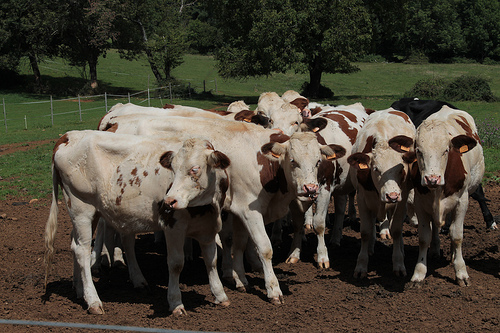
\includegraphics[scale=.4]{figures/2410240}}

\hspace{-.2cm}\fbox{\begin{minipage}{18.35em}
\textcolor{red}{DESCRIPTION}: there are two cows standing in the field. there are trees behind them.
\end{minipage}}
\vspace{.5cm}

\textbf{How well do you agree with the following statements?}
     
\begin{enumerate}
\item The description contains words that correctly refer to the objects and events in the image

\setlength{\fboxsep}{5pt}
\fbox{\IosSevenSlider{6cm}{0.6}}

\item The description is referring to the relevant/important parts of the image.

\setlength{\fboxsep}{5pt}
\fbox{\IosSevenSlider{6cm}{0.7}}

\item The sentences have a correct structure and are grammatical.

\setlength{\fboxsep}{5pt}
\fbox{\IosSevenSlider{6cm}{0.8}}

\item The sentences are well-connected and form a single story.

\setlength{\fboxsep}{5pt}
\fbox{\IosSevenSlider{6cm}{0.4}}

\end{enumerate}
     
Write you feedback in the field below if you have any (not necessary).

\end{document}

%%% Local Variables:
%%% mode: latex
%%% mode: flyspell
%%% TeX-master: t
%%% TeX-PDF-mode: t
%%% coding: utf-8
%%% ispell-local-dictionary: "british"
%%% End: